\documentclass{article}

% Packages
\usepackage{geometry}
\usepackage{graphicx}
\usepackage{lipsum}
\usepackage{listings}
\usepackage[portuguese]{babel}

% -- Defining colors:
\usepackage[dvipsnames]{xcolor}
\definecolor{codegreen}{rgb}{0,0.6,0}
\definecolor{codegray}{rgb}{0.5,0.5,0.5}
\definecolor{codepurple}{rgb}{0.58,0,0.82}
\definecolor{backcolour}{rgb}{0.95,0.95,0.92}

% Definig a custom style:
\lstdefinestyle{mystyle}{
    backgroundcolor=\color{backcolour},   
    commentstyle=\color{codepurple},
    keywordstyle=\color{NavyBlue},
    numberstyle=\tiny\color{codegray},
    stringstyle=\color{codepurple},
    basicstyle=\ttfamily\footnotesize\bfseries,
    breakatwhitespace=false,         
    breaklines=true,                                   
    keepspaces=true,                 
    numbers=left,                    
    numbersep=5pt,                  
    showspaces=false,                
    showstringspaces=false,
    showtabs=false,                  
    tabsize=2,
    captionpos=b
}

% -- Setting up the custom style:
\lstset{style=mystyle}

% Page setup
\geometry{a4paper, margin=2cm}

\begin{document}

% cover
\thispagestyle{empty} % Remove page number from first page

\begin{figure}[t]
    
\includegraphics[width=3cm]{images/logo-puc-minas.png}
    \hspace{0.02\textwidth}
    \vline%
    \hspace{0.04\textwidth}
    
\includegraphics[width=3cm]{images/logo-icei.jpeg}
\end{figure}

\hrulefill%
\vspace{\baselineskip}

\Large\noindent
\textbf{Pontifícia Universidade Católica de Minas Gerais} \\
\textbf{Instituto de Ciências Exatas e Informática} \\
\textbf{Departamento de Engenharia de Computação}

\begin{center}
    \vfill
    \Huge\textbf{Relatório: Trabalho Prático 2} \\
    \vspace{0.5cm}
    \Large\textbf{Registradores em VHDL} \\
    \vspace{1cm}
    \large \textbf{Professor(es)}: Antônio Hamilton Magalhães\\
    \vspace{0.5cm}
    \large \textbf{Aluno(s)}: Bruno Luiz Dias Alves de Castro \\
    \large \hspace{0.75cm} Rafael Ramos de Andrade \\
    \vfill
    \large Belo Horizonte \\ Campus Coração Eucarístico \\
    \vspace{\baselineskip}
    \large \today
\end{center}

% table of contents
\newpage
\thispagestyle{empty}
\tableofcontents

% body
\newpage
\large % document text size

\section{Introdução}

Durante as aulas da disciplina de Sistemas Reconfiguráveis, fomos introduzidos à linguagem VHDL. VHDL (\textbf{V}HSIC \textbf{H}ardware \textbf{D}escription \textbf{L}anguage) é uma linguagem de descrição de hardware. Com ela, podemos montar circuitos lógicos de maneira totalmente textual, o que garante à linguagem uma grande vantagem ante à soluções visuais.

\subsection{Objetivos}

\subsection{Simulação via Quartus II}

Nessa etapa realizamos testes no software Quartus II da altera.

\subsubsection{Bloco w\_reg}

Nesta imagem é realizado 3 testes para verificar a funcionalidade do registrador, nos primeiros 60ns é alterado os bits da entrada de dados (d\_in) para nivel lógico alto, o bit de reset (nrst) que é ativo em baixa, é desativado, ou seja, nível lógico alto e o bit de ativação (wr\_en) é colocoado em nível lógico alto após 10ns. Assim é possível verificar a mudança na saída (w\_out) com um tempo de delay de 6ns. No segundo teste a partir de 60ns até 140ns é resetado os bits da memória do registrador colocando reset em nível lógico zero, o resultado é propagada para a saída após o tempo de delay de aproximadamente 6ns. No terceiro teste foi verificados se o bit de ativação de escrita está funcionando corretamente, portanto com o bit 6 da saída em nível lógico alto esse valor será escrito apenas no tempo 160ns quando é colocado a porta de ativação do registrador em nível lógico alto e o registrador é escrito.

\begin{figure}[ht]
\begin{center}
    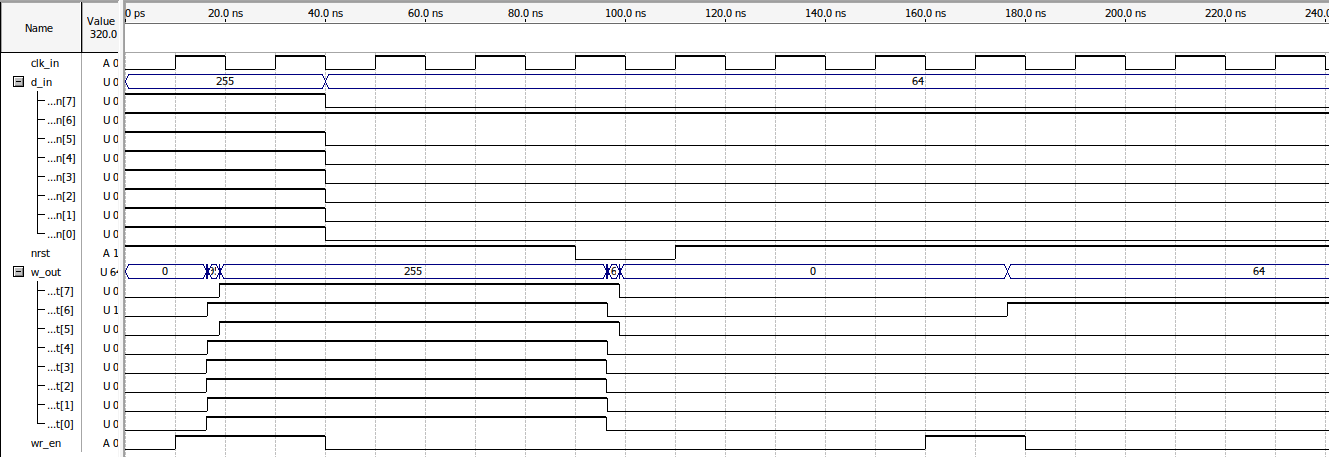
\includegraphics[width=15cm]{images/w_reg.png}
    \caption{Simulação bloco w\_reg}
\end{center}
\end{figure}

\section{fsr\_reg}

O registrador FSR é um registrador semelhante ao implemntado anteriormente. A principal diferença entre os dois está na presença de um sistema de endereçamento, e de duas entradas binárias independentes para habilitação da escrita e da leitura. Os requisitos são descritos na tabela abaixo.

\begin{center}
\begin{tabular}{|c|c|c|c|}
        \hline
        Nome & Tamanho & Tipo & Descrição\\
        \hline
        nrst & 1 bit & \textit{Input} & Entrada de \textit{reset} assíncrono.\\
        \hline
        clk\_in & 1 bit & \textit{Input} & Entrada de \textit{clock}.\\
        \hline
        abus\_in & 9 bit & \textit{Input} & Entrada de enderençamento\\
        \hline
        dbus\_in & 8 bits & \textit{Input} & Entrada de dados para escrita\\
        \hline
        wr\_sel & 1 bit & \textit{Input} & Entrada de habilitação de escrita\\
        \hline
        rd\_sel & 1 bit & \textit{Input} & Entrada de habilitação de leitura\\
        \hline
        dbus\_out & 8 bits & \textit{Output} & Saída de dadas hailitada por rd\_en\\
        \hline
        fsr\_out & 8 bits & \textit{Output} & Saída de dadas dados sempre ativa\\
        \hline
\end{tabular}
\end{center}

\subsection{Implementação}

O registrador fsr\_reg foi implementado utilizando a linguagem VHDL.\\

O código na íntegra está abaixo:\\

\begin{lstlisting}[language=VHDL, caption={Código VHDL fsr\_reg}]
LIBRARY ieee;
USE ieee.std_logic_1164.all;
USE ieee.std_logic_unsigned.all;
USE ieee.numeric_std.all;

ENTITY fsr_reg IS
    PORT (
        -- Inputs
        nrst : IN STD_LOGIC;                            -- Reset
        clk_in: IN STD_LOGIC;                           -- Clock
        abus_in: IN STD_LOGIC_VECTOR(8 DOWNTO 0);       -- Enderecamento
        dbus_in: IN STD_LOGIC_VECTOR(7 DOWNTO 0);       -- Dados
        wr_en : IN STD_LOGIC;                           -- Enable escrita
        rd_en : IN STD_LOGIC;                           -- Enable leitura

        -- Outputs
        dbus_out : OUT STD_LOGIC_VECTOR(7 DOWNTO 0);    -- Dados
        fsr_out : OUT STD_LOGIC_VECTOR(7 DOWNTO 0)      -- Registrador
    );
END ENTITY;

ARCHITECTURE fsr_reg OF fsr_reg IS
    SIGNAL mem_reg: STD_LOGIC_VECTOR(7 DOWNTO 0);
BEGIN
    PROCESS (nrst, clk_in, mem_reg, abus_in, dbus_in)
    BEGIN
        IF nrst = '0' THEN
            mem_reg <= "00000000";
        ELSIF abus_in(6 DOWNTO 0) = "0000100" THEN
            IF RISING_EDGE(clk_in) THEN
                IF wr_en = '1' THEN
                    mem_reg <= dbus_in;
                END IF;
            END IF;
        END IF;
    END PROCESS;

    dbus_out <= mem_reg WHEN rd_en = '1' ELSE "ZZZZZZZZ";
    fsr_out <= mem_reg;
END fsr_reg;    
\end{lstlisting}

\subsection{Simulação}

Para testar nosso código VHDL e certificar-nos de que nosso circuito funciona de maneira esperada, simulamos alguns casos de testes utilizando o software Quatus II.\\

Os testes realizados foram os seguites:

\begin{enumerate}
    \item Escrita com enderaçamento incorreto (diferente de XX0000100).
    \begin{itemize}
        \item \textbf{Comportamento esperado:}
        \begin{itemize}
            \item dbus\_out em alta impedância;
            \item fsr\_out sem alteração;
        \end{itemize}
    \end{itemize}
    
    \item Leitura habilitada e escrita desabilitada.
    \begin{itemize}
        \item \textbf{Comportamento esperado:}
        \begin{itemize}
            \item dbus\_out = frs\_out = último valor escrito;
        \end{itemize}
    \end{itemize}

    \item Leitura desabilitada e escrita habilitada.
    \begin{itemize}
        \item \textbf{Comportamento esperado:}
        \begin{itemize}
            \item dbus\_out em alta impendância;
            \item frs\_out = dbus\_in;
        \end{itemize}
    \end{itemize}

    \item \textit{Reset} com leitura habilitada.
    \begin{itemize}
        \item \textbf{Comportamento esperado:}
        \begin{itemize}
            \item dbus\_out = frs\_out = ``0b00000000'';
        \end{itemize}
    \end{itemize}
\end{enumerate}

\begin{figure}[ht]
    \begin{center}
        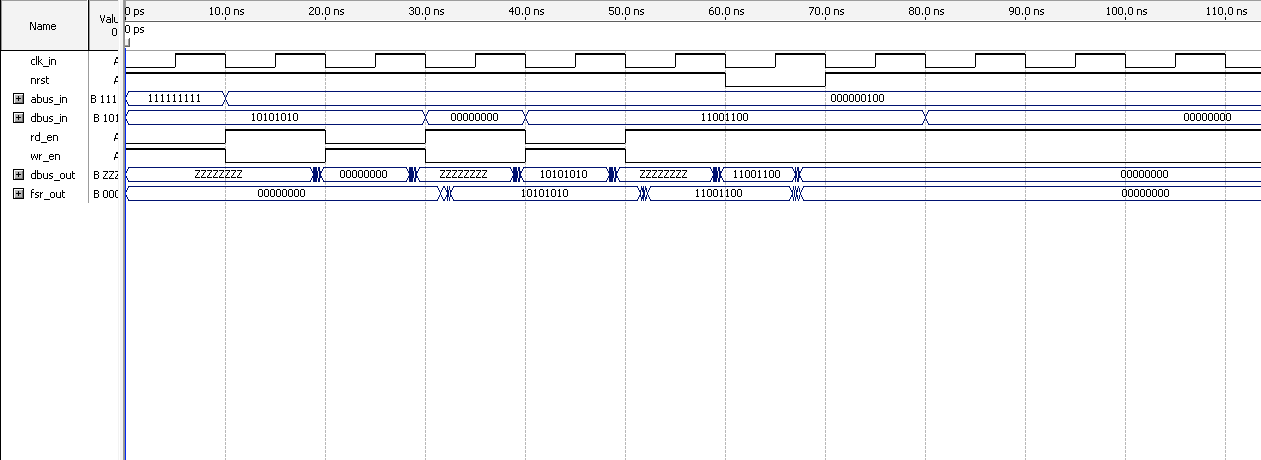
\includegraphics[width=15cm]{images/fsr_reg.png}
        \caption{Simulação fsr\_reg}
\end{center}
\end{figure}

\section{Conclusão}
Com estes dois projetos simples, tivemos um excelente primeiro contado com a linguagem VHDL, bem como à programação concorrente e desenvolvimento de circuitos FPGA. Os dois circuitos implementados (Multiplexador de Endereçamento e Unidade Lógica Aritimética) são blocos de construção chave para a maior parte dos circuitos complexos, e serão de suma importância não só para os demais trabalhos práticos que realizaremos ao longo do semestre, mas para nosso desenvolvimento acadêmico e profissional.

\end{document}
